\documentclass[../main.tex]{subfiles}

\begin{document}
    \chapter{Meta-learners} \label{ch:metalearners}
    Com alguns dels mètodes anteriors, els meta-learners sorgeixen amb l’augment de la potència computacional ha permès que des del Machine Learning, es desenvolupessin models capaços d’aconseguir molt bones prediccions mitjançant l’entrenament. Tanmateix, en el context de la inferència causal l’objectiu no és només fer prediccions, sinó respondre a la pregunta: “què passa si...?” (\citealp{hernan2020}). \par
    En aquest cas, els meta-learners aborden aquesta dificultat utilitzant l’aprenentatge automàtic per generar prediccions (els tres algoritmes que es presenten poden aprofitar qualsevol mètode supervisat de ML) per construir pseudo-outcomes.  D’aquesta manera es busca superar el problema fonamental de no disposar d'observacions amb i sense tractaments (en el cas binari) per calcular el CATE (\citealp{facure2022}). Un problema que també dificultarà avaluar la validesa dels resultats, amb dades reals serà pràcticament impossible. \par
    La idea clau és modelar tant el resultat factual (amb el tractament realment aplicat) com el contrafactual (amb el tractament alternatiu) per a cada individu, és a dir, què hauria passat si hagués rebut o no el tractament, i, a partir d’aquestes dues prediccions, estimar el CATE. L’estudi de \cite{kunzel2019} constitueix la referència fonamental sobre aquests meta-learners i és la font principal del contingut que es presenta en les tres seccions següents.


    \section{S-learner} \label{sec:slearner}
     El meta-learner més senzill és el S-learner. El seu nom prové de Single, ja que utilitza un únic model predictiu per estimar el resultat esperat, tractant el tractament T com una covariable més. Aquest model s’utilitza per generar els pseudo-outcomes necessaris per al càlcul del CATE. El seu funcionament es pot captar si ens fixem el seu algoritme que és el següent:
    
    \begin{table}[H]
        \begin{minipage}{\linewidth}
            \begin{algorithm}[H]
            \caption{\textbf{Pseudocodi S-learner} $(X,Y,T)$}
            \begin{algorithmic}[1]
              \State Estimar $\hat{\mu}(x,t) = M(Y \sim X, T)$
              \State Calcular $\hat{\tau}_S(x) = \hat{\mu}(x,1) - \hat{\mu}(x,0)$
            \end{algorithmic}
            \end{algorithm}
            \vspace{-3ex}
            {\scriptsize\textit{$\mu(x,t) = M(Y \sim X, T)$ estima $\mathbb{E}[Y_{obs} \mid X = x, T = t]$ on $t\in(0,1)$}}
        \end{minipage}
    \end{table}

    El pseudocodi mostra clarament que el procés consta només de dues fases: l'entrenament del model i el càlcul del CATE. La figura \ref{fig:sl} ho representa visualment, destacant amb línies discontínues la fase d’entrenament i, posteriorment, la utilització del model conjuntament amb les dades per calcular les $\hat{\tau}(x)$.
    
    \begin{figure}[H]
        \centering
        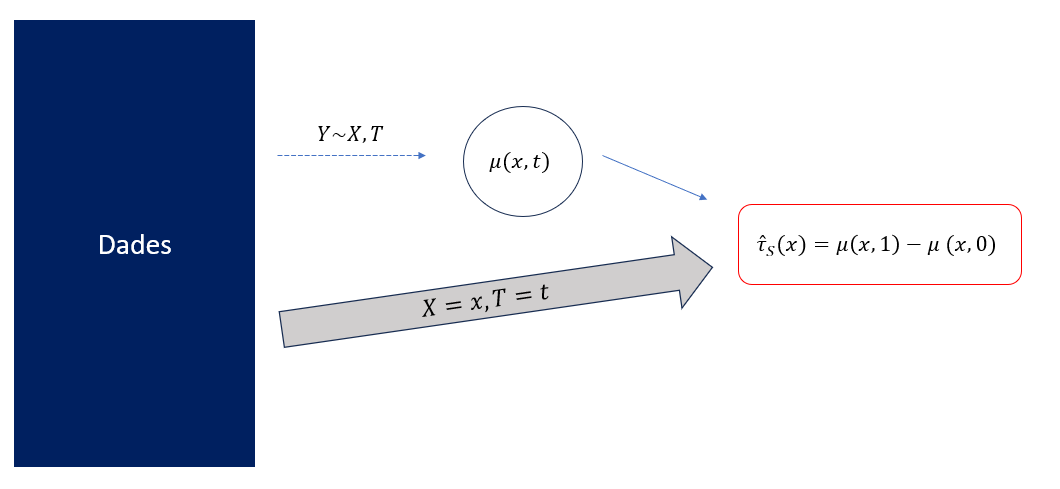
\includegraphics[width=0.8\linewidth]{imgs/s-learner.png}
        \caption{Esquema del funcionament del S-learner. D'elaboració pròpia.}
        \label{fig:sl}
    \end{figure}

    Aquest primer mètode és senzill i, per tant, fàcil d’implementar. Un dels seus punts forts és que, com utilitza totes les dades disponibles, pot ser relativament estable fins i tot en mostres petites. A més, resulta especialment eficient quan l’efecte del tractament (CATE) és petit o gairebé constant.\par
    No obstant això, també presenta limitacions importants. Pot estar esbiaixat cap a zero si el model no capta correctament la interacció entre les covariables i el tractament, ja que pot acabar ignorant o infravalorant la seva influència de T. Això el fa poc adequat quan l’efecte del tractament és heterogeni i complex.

    
    \section{T-learner} \label{sec:tlearner}
    Igual que el model anterior rep la S de "Single", aquest pren la T de "Two" perquè es basa en l’entrenament de dos models separats ($\mu_0$ i $\mu_1$), un per cada grup de tractament. Aquesta estratègia introdueix una mica més de complexitat, però també més flexibilitat per capturar diferències entre grups. El funcionament bàsic es pot veure clarament en l’algoritme i l’esquema següents.
    
    \begin{table}[H]
        \begin{minipage}{\linewidth}
            \begin{algorithm}[H]
            \caption{\textbf{Pseudocodi T-learner} $(X,Y,T)$}
            \begin{algorithmic}[1]
              \State Estimar: 
                    \begin{itemize}
                        \item[] $\hat{\mu}_0(x) = M_t(Y^t \sim X^t)$
                        \item[] $\hat{\mu}_1(x) = M_1(Y \sim X \mid T = 1)$
                      \end{itemize}
              \State Calcular $\hat{\tau}_S(x) = \hat{\mu}_1(x) - \hat{\mu}_0(x)$
            \end{algorithmic}
            \end{algorithm}
            \vspace{-3ex}
            {\scriptsize\textit{Els exponents de $X$ i $Y$ fan referència al tractament del subgrup utilitzat. Quan $T=t$, podem expressar $\hat{\mu}_t$ com $ M_t(Y \sim X \mid T = t)$}}
        \end{minipage}
    \end{table}

    Tant l’algoritme com la figura \ref{fig:tl} il·lustren amb claredat l’element més distintiu d’aquest meta-learner: es construeixen dos models independents, un per a cada grup de tractament. Cada model s’entrena només amb les dades del seu subgrup i s’utilitza per generar pseudo-outcomes, que actuen com a estimacions dels resultats potencials corresponents. A partir d’aquestes prediccions, i en funció de les covariables $X$, es calcula una aproximació al CATE.
    
    \begin{figure}[H]
        \centering
        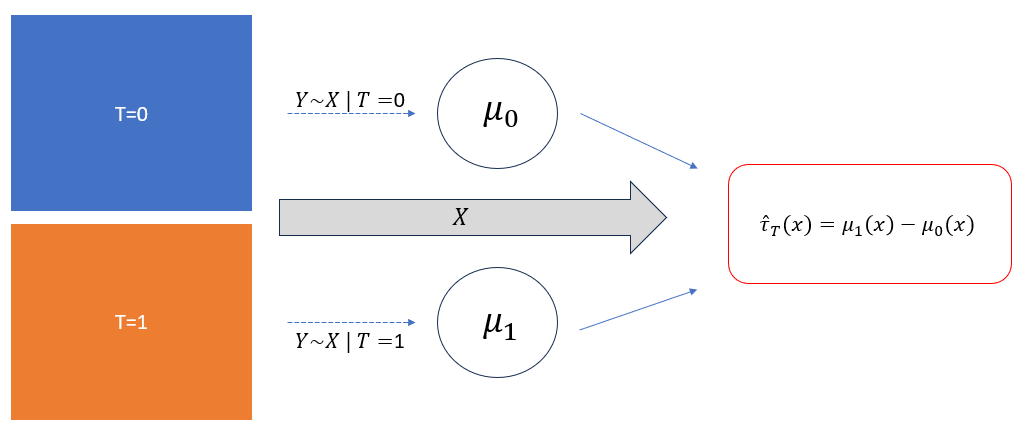
\includegraphics[width=0.8\linewidth]{imgs/t-learner.png}
        \caption{Esquema del funcionament del T-learner. D'elaboració pròpia.}
        \label{fig:tl}
    \end{figure}

    Aquest mètode continua essent senzill i alhora molt flexible, ja que permet captar millor les diferències en els pseudo-outcomes, especialment quan la distinció entre el grup tractat i el de control és rellevant.\par
    Tanmateix, també presenta algunes limitacions. Si algun dels grups (tractament o control) és petit, pot generar una alta variància en les estimacions, cosa que afecta negativament la precisió del CATE. A més, la seva robustesa disminueix quan els resultats potencials tenen una estructura complexa.\par
    Un altre inconvenient important és que el T-learner no comparteix informació entre tractats i no tractats, fet que comporta una pèrdua d’eficiència en escenaris amb mostres desequilibrades.


    \section{X-learner} \label{sec:xlearner}
    Finalment, el X-learner és el més complex dels tres meta-learners, ja que incorpora diverses fases d’estimació encadenades. Comença igual que el T-learner, amb la construcció de dos models separats per als grups tractat i control, però després utilitza aquests models per generar estimacions individuals de l’efecte del tractament a partir de prediccions contrafactuals. Aquestes diferències s’utilitzen per entrenar models específics, que combinats mitjançant una funció de pes (com ara la propensity score), permeten obtenir una estimació del CATE.
    
    \begin{table}[H]
        \begin{minipage}{\linewidth}
            \begin{algorithm}[H]
            \caption{\textbf{Pseudocodi X-learner}$(X,Y,T,g)$}
            \begin{algorithmic}[1]
                \State Estimar: 
                    \begin{itemize}
                        \item[] $\hat\mu_0 = M_0(Y^0 \sim X^0)$
                        \item[] $\hat\mu_1 = M_1(Y^1 \sim X^1)$
                    \end{itemize}
                    
                \State Calcular:
                  \begin{itemize}
                    \item[] $\tilde{D}_1^i = Y_i^1 - \hat\mu_0(X_i^1)$
                    \item[] $\tilde{D}_0^i = \hat\mu_1(X_i^0) - Y_i^0$
                  \end{itemize}
                  
                \State Estimar:
                  \begin{itemize}
                    \item[] $\hat{\tau}_1 = M_{T_1}(\tilde{D}_1^i \sim X^1)$
                    \item[] $\hat{\tau}_0 = M_{T_0}(\tilde{D}_0^i \sim X^0)$
                  \end{itemize}
                  
                \State Calcular $\hat{\tau}(x) = g(x)\hat{\tau}_0(x) + (1 - g(x))\hat{\tau}_1(x)$
            \end{algorithmic}
            \end{algorithm}
            \vspace{-3ex}
            {\scriptsize\textit{La funció de pes $g(x) \in [0,1]$ s’utilitza per minimitzar la variància de $\hat{\tau}(x)$. Una opció habitual, que sovint ofereix bons resultats, és emprar la propensity score.}}
        \end{minipage}
    \end{table}

    Un cop vist l’algoritme, la figura \ref{fig:xl} ens ajuda a completar la comprensió del funcionament del X-learner. La seva primera fase és idèntica a la del T-learner, amb l’estimació dels models $\hat{\mu}_0(x)$ i $\hat{\mu}_1(x)$ per a cada grup de tractament.\par
    A partir d’aquests models, es calculen unes pseudo-diferències entre el resultat observat i l’estimació del contrafactual. Aquestes diferències s’utilitzen per entrenar dos nous models que, un cop ponderats mitjançant una funció de pes, permeten calcular $\hat{\tau}(x)$, és a dir, una aproximació individual del CATE en funció de les covariables disponibles.
    
    \begin{figure}[H]
        \centering
        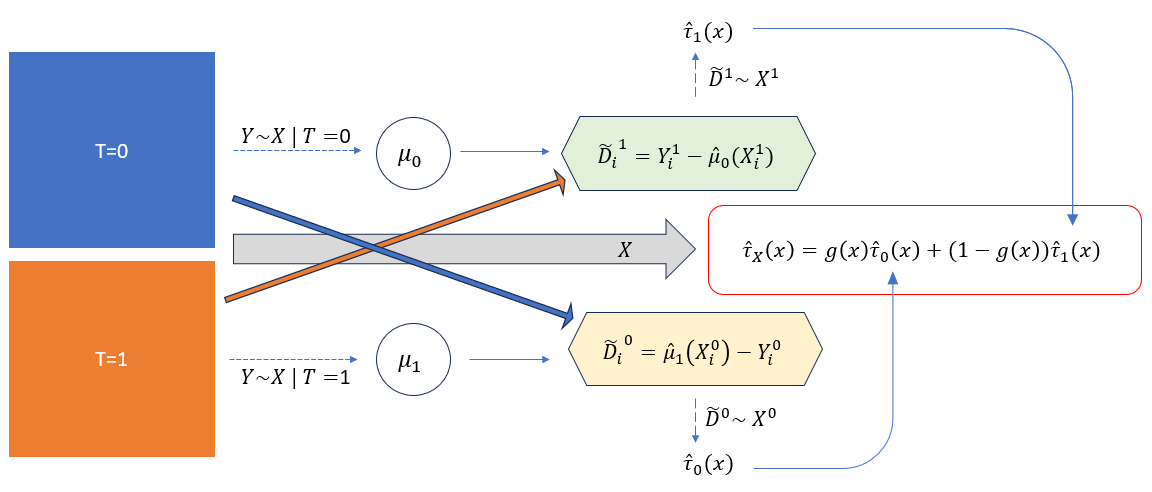
\includegraphics[width=0.8\linewidth]{imgs/x-learner.png}
        \caption{Esquema del funcionament del X-learner. D'elaboració pròpia.}
        \label{fig:xl}
    \end{figure}

    La principal fortalesa del X-learner és el seu bon rendiment en situacions on els grups de tractament i control estan desequilibrats, ja que aprofita la informació de tots dos grups per millorar l’estimació del CATE. Aquesta capacitat de compartir informació el fa més robust que altres meta-learners en contextos amb distribucions asimètriques i/o relacions complexes entre els resultats potencials.\par
    No obstant això, aquest mètode implica un augment considerable de complexitat, tant conceptual com computacional. El fet d’incloure diverses fases incrementa el risc d’acumulació d’errors i pot dificultar la seva interpretació. A més, encara que gestioni bé dades desbalancejades, pot resultar problemàtic en mostres petites, on l'estabilitat dels models es veu compromesa.


\section{Reflexió final sobre els meta-learners} \label{sec:refmeta}

Una de les conseqüències més importants de treballar en el marc de la inferència causal és el, ja mencionat, problema fonamental de la causalitat: per a cada individu, només podem observar un dels dos resultats potencials (amb o sense tractament), però mai tots dos simultàniament. Aquesta limitació implica que gairebé mai podem conèixer amb certesa l’error que cometem en estimar l’efecte del tractament, ja que no tenim accés a la veritable funció de CATE per comparar-la amb les prediccions del model.\par
Per aquest motiu, és cal conèixer bé les característiques, fortaleses i limitacions de cada meta-learner. És essencial una reflexió prèvia a tria del mètode, ja que pot condicionar profundament la qualitat de les estimacions.\par
Tot i les dificultats per validar numèricament les estimacions del CATE en dades reals existeixen aproximacions útils per avaluar el rendiment dels models. En contextos sintètics, on es coneix l'efecte real, es poden calcular mètriques com l’EMSE o la PEHE, que quantifiquen directament l’error de les estimacions.\par
En entorns reals, com ara assajos clínics o estudis observacionals, s’empren estratègies indirectes, com ara la validació creuada, l’anàlisi de l’estabilitat per subgrups, o l’estimació de funcions de risc causal com el R-loss. Aquestes tècniques sovint es combinen amb mètodes com el cross-fitting, que ajuden a evitar el sobreajustament i milloren la validesa estadística de les avaluacions.\par

És important recordar que els meta-learners són una eina relativament recent. L’article de \cite{kunzel2019}, que introdueix el S-, T- i X-learner, és de fa pocs anys, i des de llavors el camp ha evolucionat ràpidament amb noves propostes metodològiques. Entre aquestes destaquen el R-learner (\cite{nie2021r}) i el DR-learner (\cite{kennedy2020dr}), que busquen millorar la fiabilitat i eficiència de les estimacions del CATE mitjançant formulacions estadísticament més sofisticades, augmentant també la complexitat i els costos computacionals.\par
El \textbf{DR-learner} es basa en el principi de doble robustesa, que consisteix a combinar dues estimacions independents (habitualment la propensity score i la mitjana condicional del resultat) de manera que si almenys una de les dues és consistent, l’estimació final del CATE també ho serà. A més, utilitza estimadors ortogonals, que són poc sensibles a petits errors en els components intermedis i redueixen així el risc d’acumulació d’error.\par
Per la seva banda, el \textbf{R-learner} reformula l’estimació del CATE com un problema de regressió de residus ponderats\footnote{La regressió de residus ponderats estima l’efecte causal ajustant els resultats i el tractament per les covariables, i regressa els residus resultants ponderats pel propensity score.}, fet que permet aplicar tècniques modernes de regularització i optimització. Tot i no ser doblement robust en el mateix sentit que el DR-learner, ofereix propietats quasi-òptimes i una gran flexibilitat pràctica.\par


En definitiva, aquest treball s’ha centrat en una primera aproximació al problema de la inferència causal amb tractaments heterogenis mitjançant meta-learners. És un punt de partida sòlid dins d’un camp que encara és actiu, viu i en creixement. Per tant, entendre bé aquestes eines, les seves aplicacions i limitacions és una base fonamental de la inferència causal.

    
\end{document}